
\documentclass[border=10pt, 12pt]{standalone}
\usepackage[svgnames]{xcolor}
\usepackage{amsmath}
\usepackage{pgfplots}
\pgfplotsset{compat=newest}
\usepackage[sfdefault]{FiraSans}
\usepackage{FiraMono}
\renewcommand*\familydefault{\sfdefault}
\begin{document}
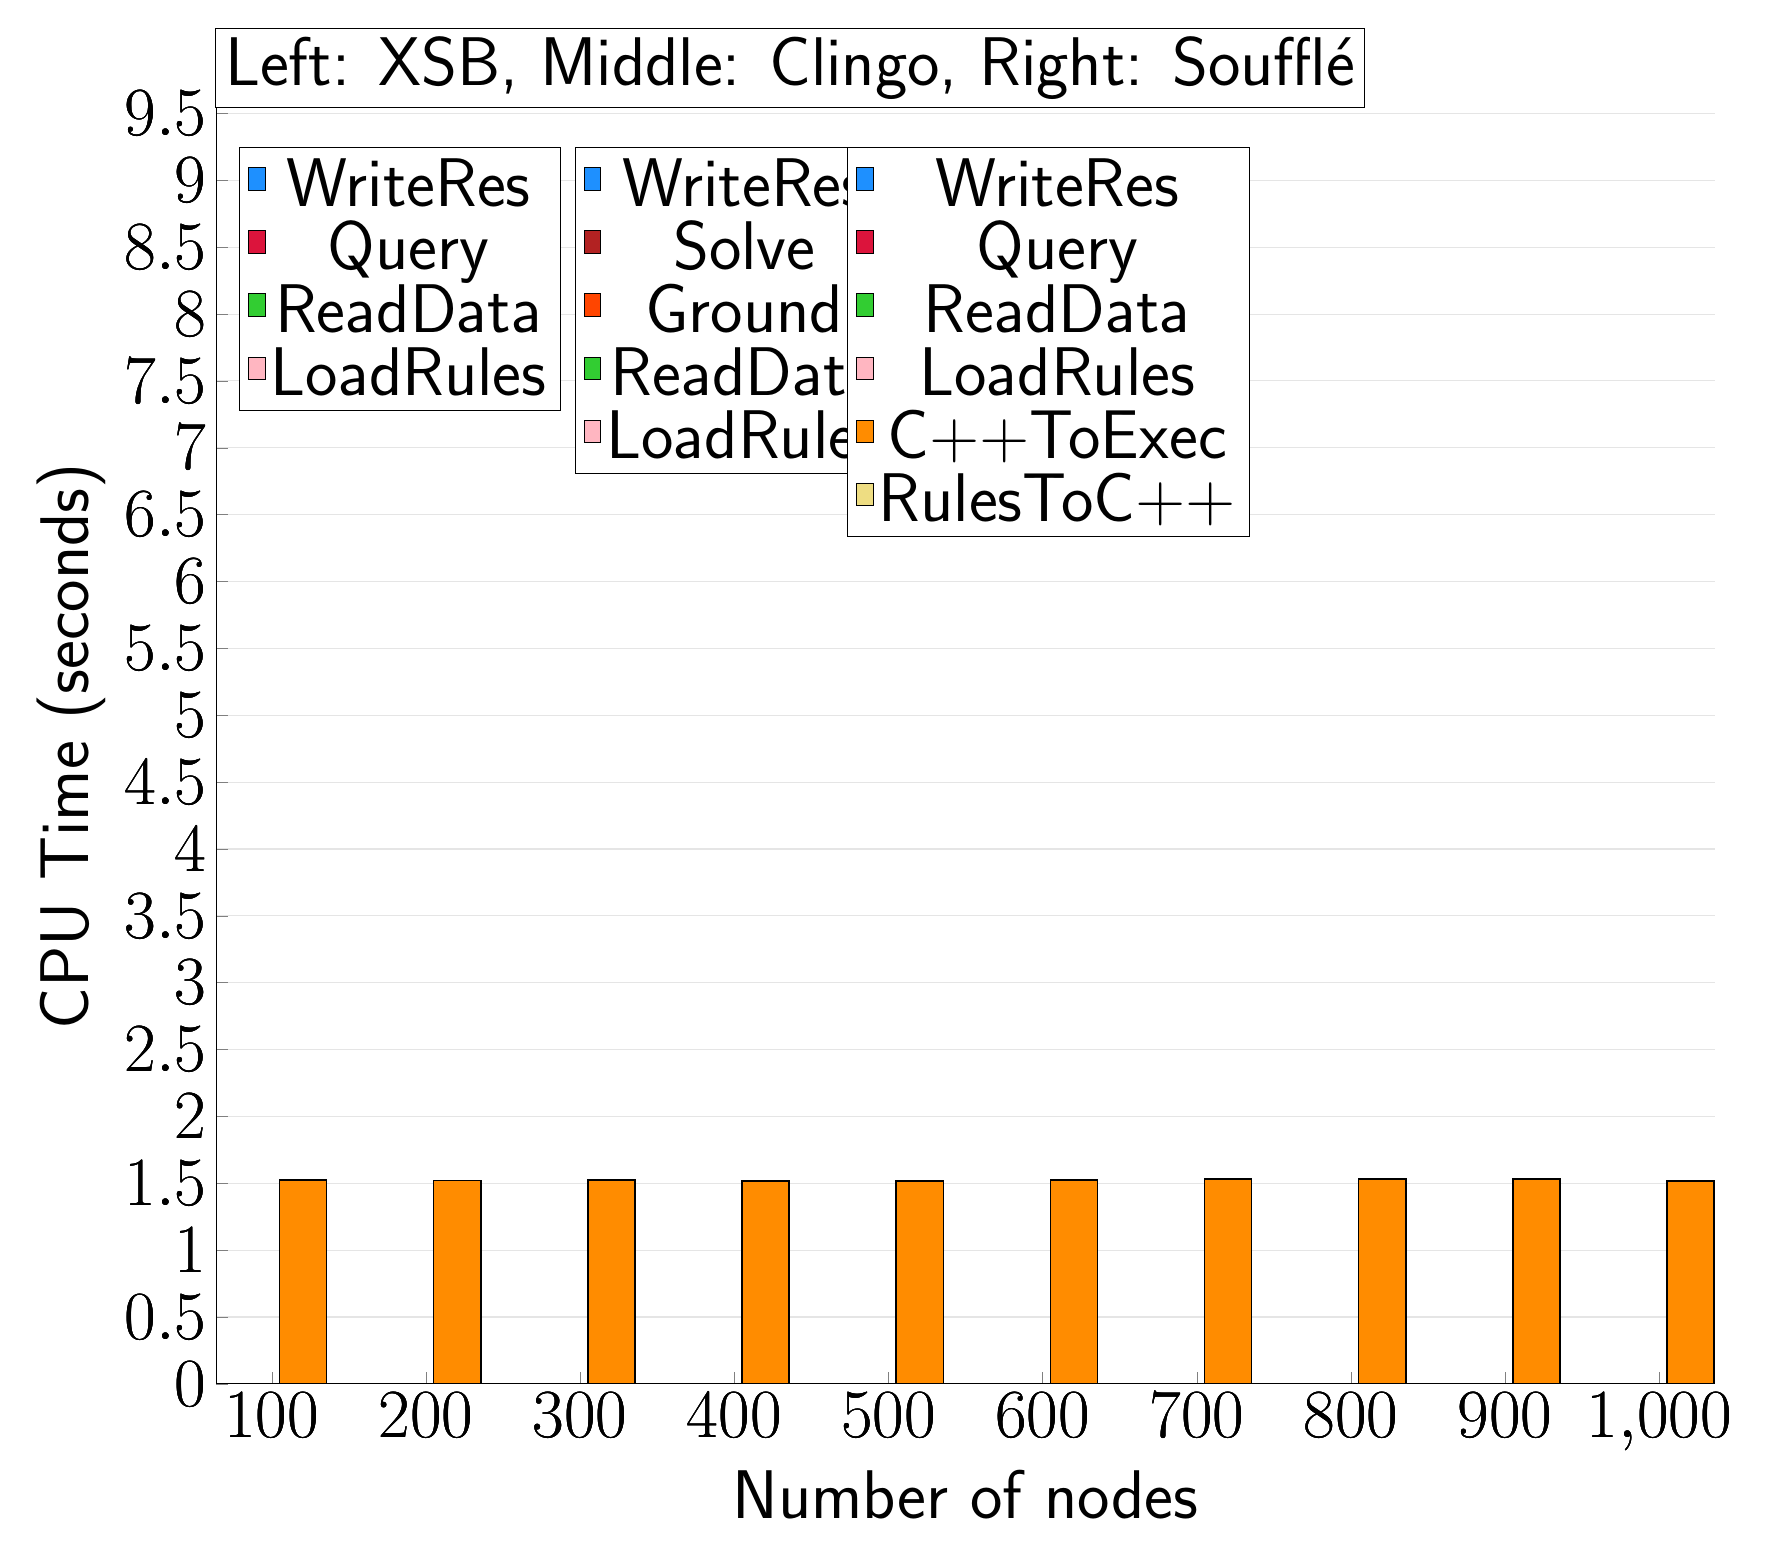
\begin{tikzpicture}
                        \begin{axis}[bar shift=-24.3pt, 
   ybar stacked,
   width=1.7\textwidth,
   bar width=0.6cm,
   ymajorgrids, tick align=inside,
   major grid style={draw=gray!20},
   xtick=data,
   ymin=0, ymax=9.538,
   axis x line*=bottom,
   axis y line*=left,
   enlarge x limits=0.04,
   legend style={
       at={(0.23, 0.97)},
       anchor=north east,
       legend columns=1,
       font=\Huge,
   },
   ylabel={CPU Time (seconds)},
   xlabel={Number of nodes},
   label style={font=\Huge},
   tick label style={font=\Huge},
]
\addlegendimage{fill=DodgerBlue, draw=black, line width=0.2pt}
\addlegendentry{WriteRes}
\addlegendimage{fill=Crimson, draw=black, line width=0.2pt}
\addlegendentry{Query}
\addlegendimage{fill=LimeGreen, draw=black, line width=0.2pt}
\addlegendentry{ReadData}
\addlegendimage{fill=LightPink, draw=black, line width=0.2pt}
\addlegendentry{LoadRules}
\addplot +[fill=LightPink, draw=black, line width=0.55pt] coordinates {
(100, 0.0005639999999999997)
(200, 0.0005524000000000002)
(300, 0.0005517999999999994)
(400, 0.0005642000000000002)
(500, 0.0005568000000000006)
(600, 0.0005539999999999998)
(700, 0.0005533999999999998)
(800, 0.0005532000000000002)
(900, 0.0005513999999999999)
(1000, 0.0005502000000000005)
};
\addplot +[fill=LimeGreen, draw=black, line width=0.55pt] coordinates {
(100, 0.00019400000000000022)
(200, 0.0002697999999999998)
(300, 0.00034679999999999954)
(400, 0.00042000000000000023)
(500, 0.0005029999999999994)
(600, 0.0005666000000000002)
(700, 0.0006450000000000003)
(800, 0.0007159999999999997)
(900, 0.0007842000000000003)
(1000, 0.0008662000000000005)
};
\addplot +[fill=Crimson, draw=black, line width=0.55pt] coordinates {
(100, 3.39999999999993e-06)
(200, 3.599999999999784e-06)
(300, 3.4000000000002783e-06)
(400, 3.9999999999994924e-06)
(500, 3.4000000000002783e-06)
(600, 3.40000000000028e-06)
(700, 3.5999999999997847e-06)
(800, 3.4000000000002783e-06)
(900, 3.7999999999996384e-06)
(1000, 3.5999999999994383e-06)
};
\addplot +[fill=DodgerBlue, draw=black, line width=0.55pt] coordinates {
(100, 5.9599999999999606e-05)
(200, 5.980000000000011e-05)
(300, 6.159999999999952e-05)
(400, 6.0400000000000384e-05)
(500, 5.979999999999979e-05)
(600, 6.039999999999972e-05)
(700, 6.0200000000000196e-05)
(800, 6.0399999999999666e-05)
(900, 5.9200000000000605e-05)
(1000, 6.22000000000001e-05)
};
\end{axis}

\begin{axis}[bar shift=-6.5pt, 
   ybar stacked,
   width=1.7\textwidth,
   bar width=0.6cm,
   ymajorgrids, tick align=inside,
   major grid style={draw=none},
   xtick=data,
   ymin=0, ymax=9.538,
   axis x line*=none,
   axis y line*=none,
   enlarge x limits=0.04,
   legend style={
       at={(0.454, 0.97)},
       anchor=north east,
       legend columns=1,
       font=\Huge,
   },
   label style={font=\Huge},
   tick label style={font=\Huge},
]
\addlegendimage{fill=DodgerBlue, draw=black, line width=0.2pt}
\addlegendentry{WriteRes}
\addlegendimage{fill=FireBrick, draw=black, line width=0.2pt}
\addlegendentry{Solve}
\addlegendimage{fill=OrangeRed, draw=black, line width=0.2pt}
\addlegendentry{Ground}
\addlegendimage{fill=LimeGreen, draw=black, line width=0.2pt}
\addlegendentry{ReadData}
\addlegendimage{fill=LightPink, draw=black, line width=0.2pt}
\addlegendentry{LoadRules}
\addplot +[fill=LightPink, draw=black, line width=0.55pt] coordinates {
(100, 0.0)
(200, 0.0)
(300, 0.0)
(400, 0.0)
(500, 0.0)
(600, 0.0)
(700, 0.0)
(800, 0.0)
(900, 0.0)
(1000, 0.0)
};
\addplot +[fill=LimeGreen, draw=black, line width=0.55pt] coordinates {
(100, 0.0)
(200, 0.0)
(300, 0.0)
(400, 0.0)
(500, 0.0)
(600, 0.0)
(700, 0.0)
(800, 0.0)
(900, 0.0)
(1000, 0.0)
};
\addplot +[fill=OrangeRed, draw=black, line width=0.55pt] coordinates {
(100, 0.0)
(200, 0.0)
(300, 0.0)
(400, 0.0)
(500, 0.0)
(600, 0.0)
(700, 0.0)
(800, 0.0)
(900, 0.0)
(1000, 0.0)
};
\addplot +[fill=FireBrick, draw=black, line width=0.55pt] coordinates {
(100, 0.0)
(200, 0.0)
(300, 0.0)
(400, 0.0)
(500, 0.0)
(600, 0.0)
(700, 0.0)
(800, 0.0)
(900, 0.0)
(1000, 0.0)
};
\addplot +[fill=DodgerBlue, draw=black, line width=0.55pt] coordinates {
(100, 0.0)
(200, 0.0)
(300, 0.0)
(400, 0.0)
(500, 0.0)
(600, 0.0)
(700, 0.0)
(800, 0.0)
(900, 0.0)
(1000, 0.0)
};
\end{axis}

\begin{axis}[bar shift=11.3pt, 
   ybar stacked,
   width=1.7\textwidth,
   bar width=0.6cm,
   ymajorgrids, tick align=inside,
   major grid style={draw=none},
   xtick=data,
   ymin=0, ymax=9.538,
   axis x line*=none,
   axis y line*=none,
   enlarge x limits=0.04,
   legend style={
       at={(0.69, 0.97)},
       anchor=north east,
       legend columns=1,
       font=\Huge,
   },
   label style={font=\Huge},
   tick label style={font=\Huge},
]
\addlegendimage{fill=DodgerBlue, draw=black, line width=0.2pt}
\addlegendentry{WriteRes}
\addlegendimage{fill=Crimson, draw=black, line width=0.2pt}
\addlegendentry{Query}
\addlegendimage{fill=LimeGreen, draw=black, line width=0.2pt}
\addlegendentry{ReadData}
\addlegendimage{fill=LightPink, draw=black, line width=0.2pt}
\addlegendentry{LoadRules}
\addlegendimage{fill=DarkOrange, draw=black, line width=0.2pt}
\addlegendentry{C++ToExec}
\addlegendimage{fill=LightGoldenrod, draw=black, line width=0.2pt}
\addlegendentry{RulesToC++}
\addplot +[fill=LightGoldenrod, draw=black, line width=0.55pt] coordinates {
(100, 0.0)
(200, 0.0)
(300, 0.0020000000000000005)
(400, 0.0)
(500, 0.0)
(600, 0.0020000000000000018)
(700, 0.0020000000000000005)
(800, 0.0020000000000000005)
(900, 0.0020000000000000005)
(1000, 0.0)
};
\addplot +[fill=DarkOrange, draw=black, line width=0.55pt] coordinates {
(100, 1.5219999999999998)
(200, 1.52)
(300, 1.52)
(400, 1.516)
(500, 1.5139999999999998)
(600, 1.518)
(700, 1.526)
(800, 1.5300000000000002)
(900, 1.528)
(1000, 1.514)
};
\addplot +[fill=LightPink, draw=black, line width=0.55pt] coordinates {
(100, 0.00011360000000000001)
(200, 0.0001552)
(300, 0.00013879999999999999)
(400, 0.00014859999999999998)
(500, 0.00013700000000000002)
(600, 0.0001454)
(700, 0.0001318)
(800, 0.00015539999999999998)
(900, 0.0001362)
(1000, 0.00013700000000000002)
};
\addplot +[fill=LimeGreen, draw=black, line width=0.55pt] coordinates {
(100, 0.0007476)
(200, 0.0011845999999999998)
(300, 0.0013594)
(400, 0.0018292000000000002)
(500, 0.0021716)
(600, 0.0027548)
(700, 0.0026756)
(800, 0.0032535999999999997)
(900, 0.0033938)
(1000, 0.0040498)
};
\addplot +[fill=Crimson, draw=black, line width=0.55pt] coordinates {
(100, 0.0001874)
(200, 0.0003556)
(300, 0.00045620000000000003)
(400, 0.0006733999999999999)
(500, 0.0008437999999999999)
(600, 0.001024)
(700, 0.0010612)
(800, 0.0012808)
(900, 0.0013454)
(1000, 0.001623)
};
\addplot +[fill=DodgerBlue, draw=black, line width=0.55pt] coordinates {
(100, 0.00017140000000000002)
(200, 0.00017360000000000002)
(300, 0.0001828)
(400, 0.000246)
(500, 0.00018439999999999998)
(600, 0.0002512)
(700, 0.0001866)
(800, 0.0001938)
(900, 0.00026060000000000005)
(1000, 0.0001988)
};
\end{axis}


\node[anchor=south, draw, fill=white] at (rel axis cs:0.42,1) {\Huge Left: XSB, Middle: Clingo, Right: Soufflé};
\end{tikzpicture}
\end{document}
                    